\chapter{Introduction} % Titlul capotilului
\label{Capitolul1}

\section*{Sistem Overview}
The LHC (Large Hadron Collider) is a 27km circumference synchrotron that accelerates two counter rotating particle beams. The beams are collided at four interaction points for a contiguous period of 10-20 hours. The ATLAS detector (A Toroidal LHC ApparatuS) \citep{aad2008atlas}, designed for studying particles produced by proton-proton interactions and heavy ion collisions surrounds one of the interaction points. 

The image below presents a section of the detector which has a layered structure with the interaction point in the center of the detector. The different layers are specialized in measuring different properties of the particles as detailed in \citep{aad2008atlas}. 

\begin{figure}[ht!]
\centering
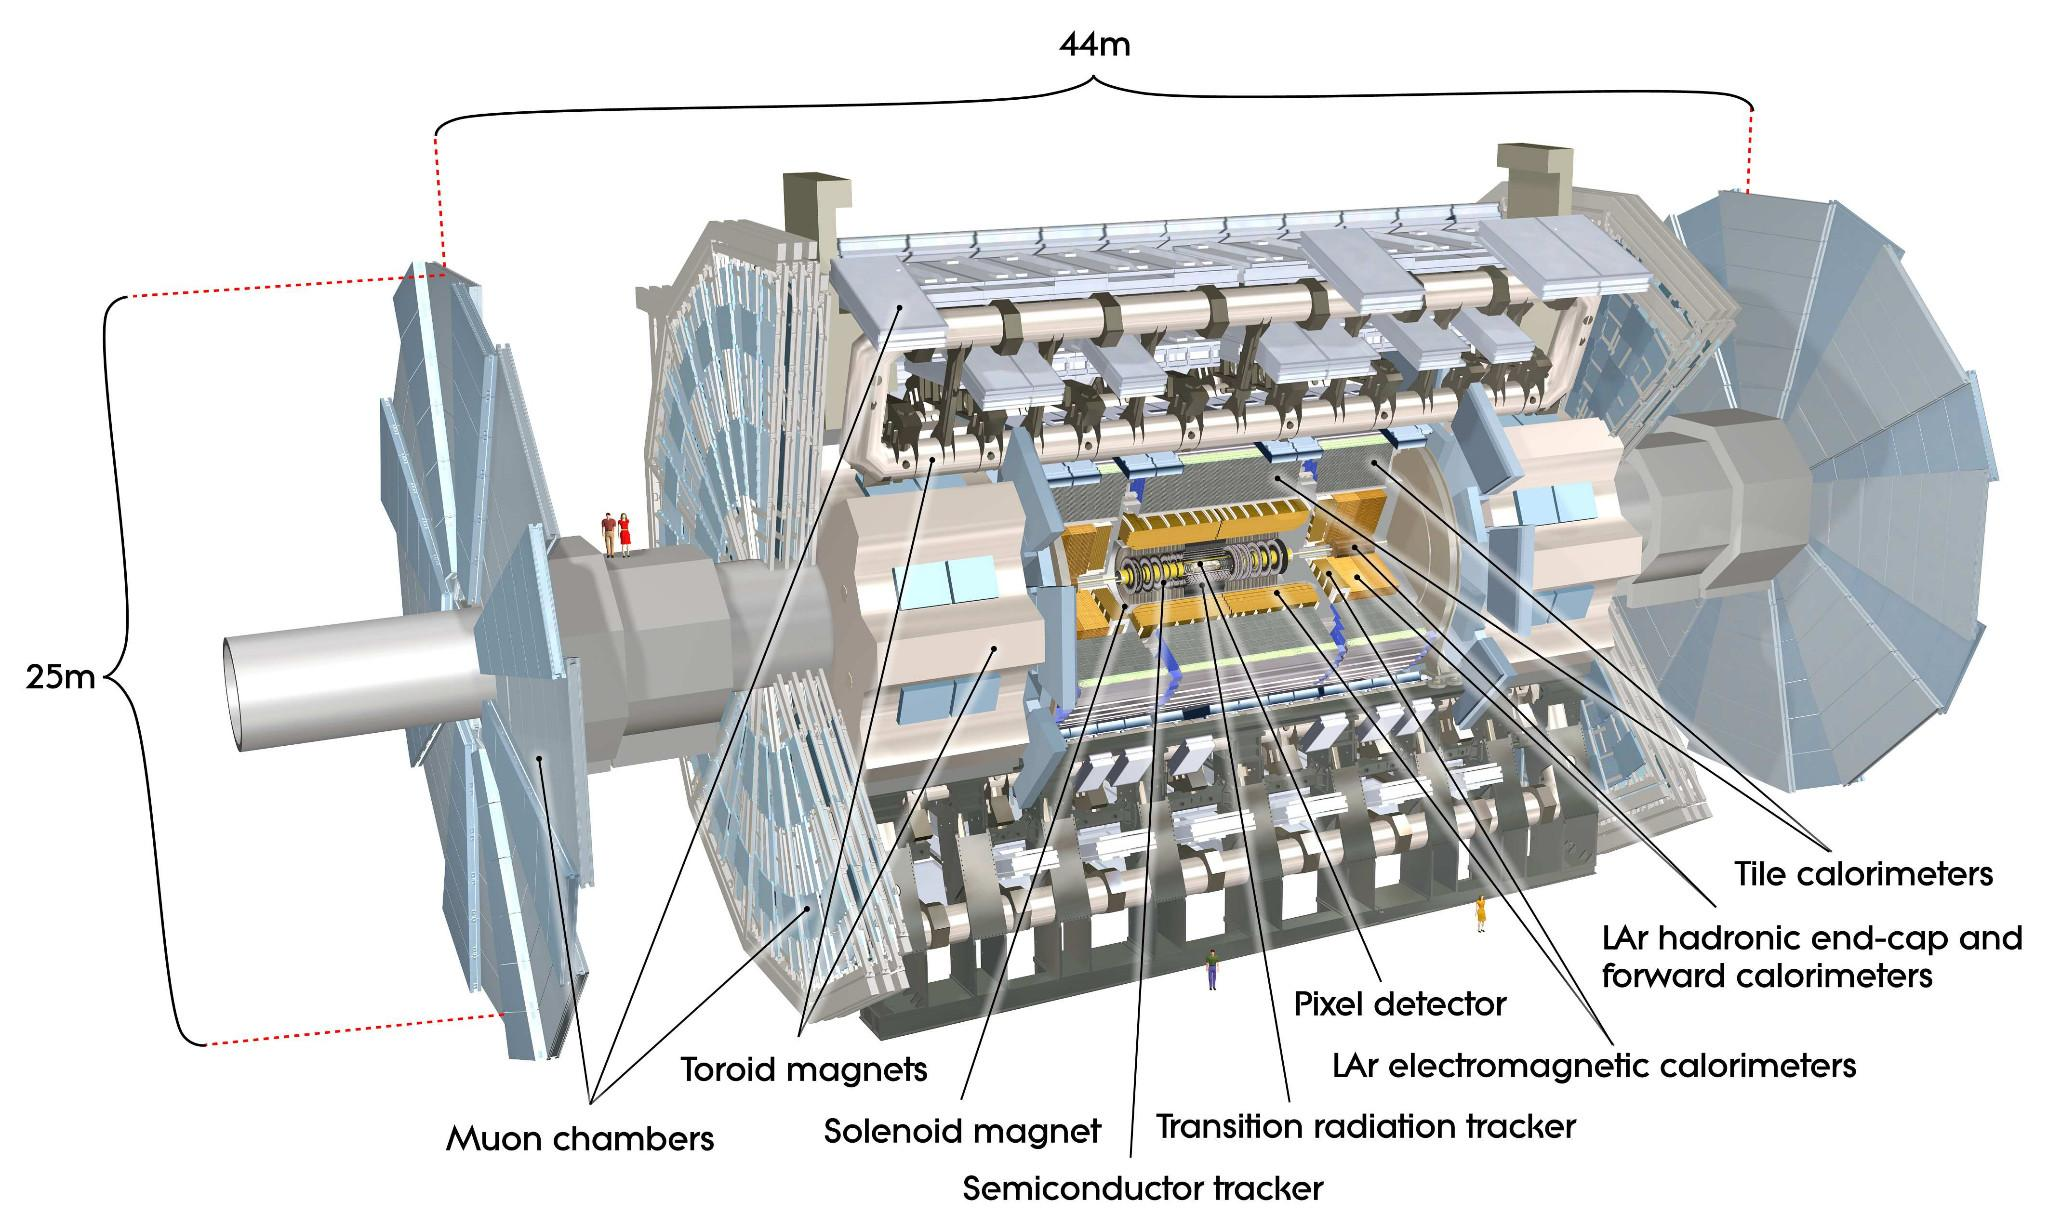
\includegraphics[scale=0.2]{Images/Overview.jpg}
\caption{ATLAS detector section view.}
\end{figure}


\section*{Event selection}
The two counter-rotating beams consist of trains of particle bunches. The distance between two consecutive particle bunches is around 25 ns and with the bunch crossing duration less than 1 ns. So bunch collision events happen with a frequency of 40MHz, each one consisting of 25 particle collisions in average. The data collected about these collisions has to be sent to the CERN persistent storage \citep{baud2003castor} for offline analysis. The amount of data collected for a single collision event is 1.5MB in average, which would mean a throughput of 60TB/s which is far more than what can be stored at a reasonable cost. Moreover, the number of events that are interesting for the offline analysis is only a small fraction of the total number of events. Hence, the events are filtered before being persisted using a three level data acquisition system (DAQ). 

\begin{figure}[ht!]
\centering
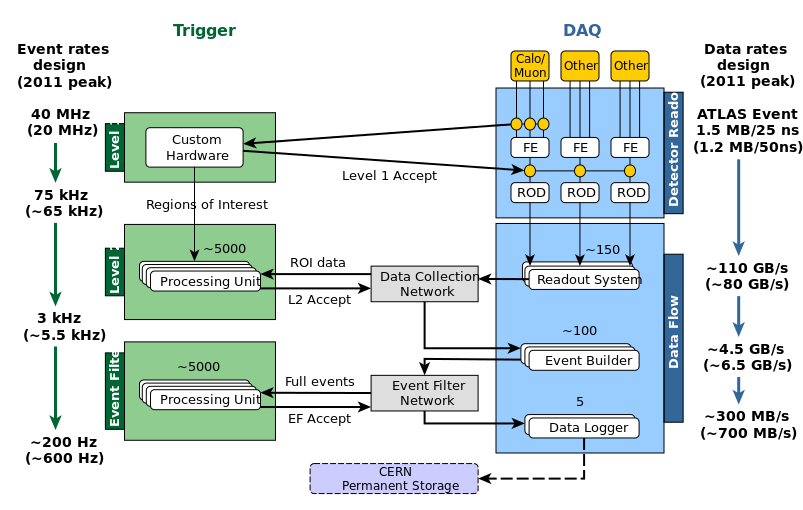
\includegraphics[scale=0.5]{Images/Trigger.png}
\caption{TDAQ system overview.}
\end{figure}

The first level trigger (L1) is built using custom hardware that can operate at 40 MHz and is placed as close to the actual detector as possible to reduce latencies caused by cable length. This level makes simple decisions based on the energy depositions in the calorimeters and of muon track segments in order to limit the latency to as low as 2.5 us. The acceptance rate of this level is chosen to be at most 75kHz. 

After being accepted by the L1, event data is stored in the ROBs (ReadOut Buffers) while it is processed by the second level trigger (L2) which is part of the HLT (High Level Trigger). The L2 reads only some parts of the data associated with an event (Regions of Interest or ROI) as hinted by the L1. The data used by the L2 system is in average 50KB per event and the latency of the order of tens of milliseconds. The L2 selection software is composed of more than 6000 instances of a software application running on 800 nodes, each of them handling one event at a time. 

Finally, the third level trigger, called Event Filter (EF) operates on the complete event data, at an input rate given by L2 of 3.5kHz. It has a configurable menu of more complicated selection algorithms and has a total latency of about 1 seconds and an acceptance rate of several hundred hertz which is within the mass storage limitations. The installation consists of 600 nodes running 6500 instances of the applications.

\subsection*{Evolution}

During the 2 year shutdown period starting at the beginning of 2013, a large upgrade of the entire system is planned \citep{hauser2012atlas}. In the DAQ system, the main change will be the merge of the L2 and EF.  

\begin{figure}[ht!]
\centering
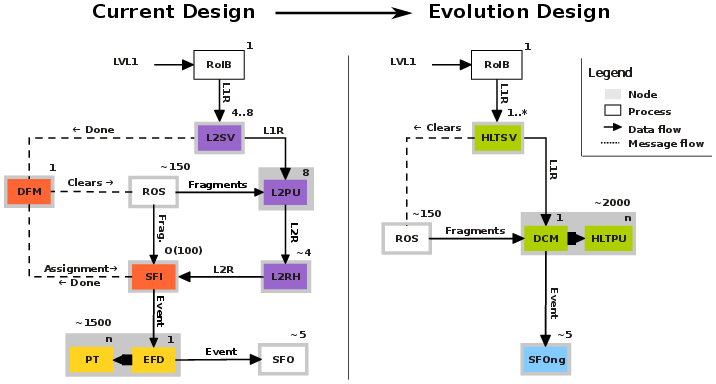
\includegraphics[scale=0.55]{Images/Evolution.png}
\caption{ATLAS TDAQ atchitecture evolution during shutdown.}
\end{figure}

All the applications dealing with event dispatching and other system management and control tasks (DFM, SFI, L2RH, EFD) will be merged into the HLT SuperVisor (HLTSV) and the DataFlow Control Manager (DCM). 
The L2 Processing Unit (L2PU) and the level 3 processing task (PT) will be merged into the HLTPU. In the new system instead of having L2 operating on chunks of event data and EF on whole events, we will have a series of algorithms that fetch event chunks incrementally as needed.

The main advantages of merging the two layers are better resource allocation, better load balancing and a simpler and more flexible system. However, assessing the benefits of this change needs validation in production mode with intensive operational monitoring.

\section*{Monitoring in ATLAS}

The ATLAS monitoring system \citep{collaboration2003atlas} is composed of information publishing libraries, information sharing services, monitoring facilities (e.g. that aggregate or persist monitoring information) and graphical displays.

There are two types of monitoring: operational monitoring which deals with operational data and functional parameters of different software and hardware components and event monitoring which monitors results of the analysis performed on events.

\subsection*{Components and services}

There are a number of components and services that play together in the monitoring system. We will present below the ones that have are the most relevant for operational monitoring starting from the lowest level ones up.

\begin{description}
\item[Inter-Process Communication (IPC) library \citep{corso2007data}] Is responsible for all the communication between applications in the ATLAS Trigger and Data AcQuisition (TDAQ)  system. It provides a much simpler interface to the underlying CORBA implementation including a simple API for the OMG Naming Service and a transparent cache for the remote object references.

\item[Object Kernel Support (OKS) database \citep{jones1998oks}\citep{alexandrov2001atlas}] Is an object-oriented database used for storing static configuration parameters for hardware and software components of the system, for example command line parameters and the node where to run a specific application. The data is loaded from XML data files and is validated against an user provided schema. 

In order to avoid overloading the database server during the system start and due to the static nature of the data, a system of caching proxies is used. This and the fact that the database does not have advanced query support enables it to meet the performance requirements of a real-time system.

\item[Partition editor] The software and hardware components in the TDAQ system are grouped in partitions which are configured using an OKS database. Due to the scale of the partitions (e.g. hundreds of applications), the configuration cannot be specified manually, but is automatically generated using a set of tools called partition editor.

\item[The ROOT framework \citep{brun1997root}] is an Object Oriented framework that contains among others an efficient file-based persistence mechanism, a C++ interpreter, reflection support, advanced statistical analysis instruments (multi dimensional histograms, fitting, minimization) and visualization tools. Most of the monitoring information in the system consists of such histograms.

\item[Information Sharing (IS) server \citep{kolosinformation}]  Is a server used to share monitoring information between applications that publish their own operational or event-related data and applications that need to process this information. The IS acts as an in memory key-value store, where keys are strings - the name of the objects - and values are subclasses of the ISInfo class. An application can read, write or update the information with a specific name. There is also the option for an application to subscribe to receive notifications when a value is updated. Due to the scale of our system, we run multiple instances of this server, each having its own name.

\begin{figure}[ht!]
\centering
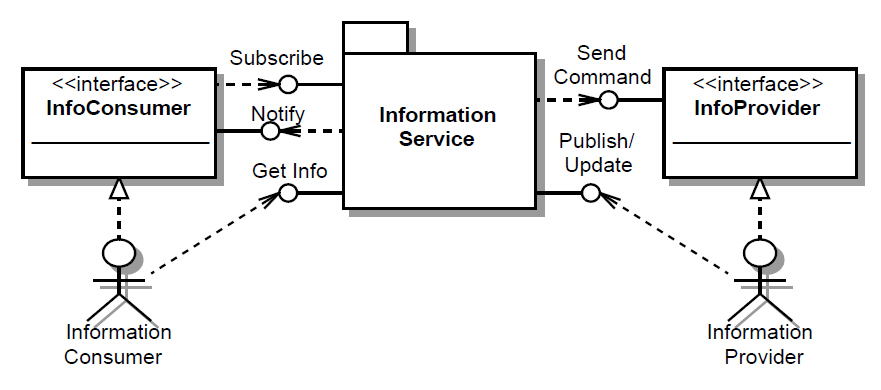
\includegraphics[scale=0.44]{Images/IS.png}
\caption{IS server interface.}
\end{figure}


The ISInfo class is intended to be a plain data structure with serialization and deserialization functions. They can be either written by the programmer or generated from an XML description.

\item[The Online Histogramming (OH) service \citep{kolosoh}] is a library which offers an interface to the IS server that allows one to store and retrieve ROOT histograms by transparently encoding them as ISInfo objects.

\item[The Gatherer \citep{renkel2010gatherer}] Is an application which aggregates monitoring information coming from different applications. For example, many applications track event data size distribution using histograms. The gatherer periodically reads all these histograms from the IS server, adds them and writes them back to the IS server. The aggregation is usually done in multiple stages, once per rack, and once globally across different IS servers. 

\item[Persistent Back-End for the AtlaS Tdaq (PBEAST) \citep{sicoe2012persistent}]: A Java application that persists operational monitoring data while storing the most recent data (1 month) in a queryable format. It subscribes to most of the IS servers and stores the updates in a Cassandra database.

\end{description}

\section*{Thesis structure}

The rest of the thesis report begins with a presentation of the project goal, namely the design and implementation of the {\tt monsvc} library. Then we describe the solutions for the challenges related to the \emph{configuration} of the library. In the next section, we present the algorithm used to \emph{schedule} the flow of monitoring information in the TDAQ network. Finally, we discuss some solutions for the \emph{synchronization} between the library which publishes the monitoring information and the application that updates it. The thesis ends with conclusions and possible future improvements.

